\documentclass[a4paper,11pt]{article}
%%%%%%%%%%%%%%%%%%%%%%%%%%%%%%%%%%%%%%%%%%%%%%%%%%%%%%%%%%%%%%%%%%%%%%%%%%%%%%%%
\usepackage{ccs_iogs}
%%%%%%%%%%%%%%%%%%%%%%%%%%%%%%%%%%%%%%%%%%%%%%%%%%%%%%%%%%%%%%%%%%%%%%%%%%%%%%%%
\begin{document}

\newpage
\begin{minipage}[c]{.25\linewidth}
	
\includegraphics[width=4cm]{images/LEnsE_IOGS.jpg}
\end{minipage} \hfill
\begin{minipage}[c]{.4\linewidth}

\begin{center}
\vspace{0.3cm}
{\Large OPTO-ELECTRONIQUE}

\medskip

\textbf{\Large TP Séance 6 / AM}

\end{center}
\end{minipage}\hfill

\begin{center}
\vspace{0.3cm}

\noindent \rule{\linewidth}{1pt}

Durée : 3h / Modulation et Démodulation / Détection synchrone

\vspace{-0.2cm}
\noindent \rule{\linewidth}{1pt}
\end{center}


%%%%%%%%%%%%%%%%%%%%%%%%%%%%%%%%%%
\section*{Objectifs de l'expérience}

On se propose dans ce TP de réaliser une démodulation d'un signal modulé, à partir d'une détection synchrone pré-câblée.

On réalisera un \textbf{étage actif de filtrage} (Partie B) permettant de récupérer le signal modulant et on validera le bon fonctionnement de la maquette de modulation/démodulation (Partie A).

	
\section*{Partie A - Etude de la modulation/démodulation \textsc{\normalsize(Durée conseillée : 60 min)}}
\subsection*{Description de la maquette}

On se propose dans cette séance d'étudier la maquette suivante permettant de faire de la modulation et de la démodulation.
On donne le schéma fonctionnel suivant :

	\begin{center}
		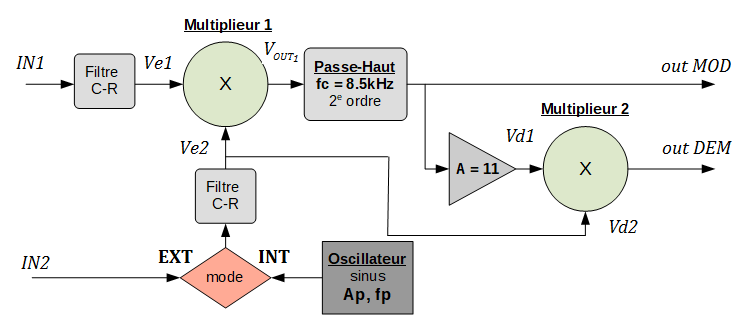
\includegraphics{images/systeme.png}
	\end{center}

L'entrée \textbf{IN1} correspond à la modulante, soit $V_m(t)$, et l'entrée \textbf{IN2} correspond à la porteuse, soit $V_p(t)$.

Le \textbf{mode} est choisi à l'aide de l'interrupteur :
\begin{itemize}
	\item	EXT : modulation par un signal externe connecté sur \textbf{IN2} ;
	\item INT : modulation par un signal interne sinusoïdal de fréquence $f_p$ et d'amplitude $A_p$.
\end{itemize}

\newpage
%%%%%%%%%%%%%%%%%%%%%%%%%%%%%%%%%%
\subsection*{A1 - Alimentation symétrique}
\parpic[r]{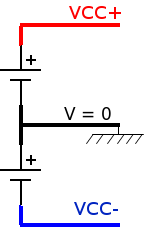
\includegraphics{./images/Alim_cablageVCC.png}}

\Real Réaliser une alimentation symétrique de +$V_{CC}$ / -$V_{CC}$ (avec $V_{CC} = 7~V$) à l'aide de l'alimentation continue composée de deux blocs indépendants (voir document annexe \textit{Description du matériel} et figure ci-contre).

\Real Proposer et mettre en oeuvre une méthode de validation de ces deux tensions (successivement).

\bigskip	
	
	\textbf{Faire valider par l'examinateur.trice.}	

%%%%%%%%%%%%%%%%%%%%%%%%%%%%%
\subsection*{A2 - Etude de l'étage multiplieur 1}



On appellera la \textbf{modulante} le signal $V_m(t) = A_m \cdot sin(2 \cdot \pi \cdot f_m \cdot t)$ (fréquence lente) sur  \textsc{\textbf{IN1}} et la \textbf{porteuse} le signal $V_p(t) = A_p \cdot sin(2 \cdot \pi \cdot f_p \cdot t)$ (fréquence rapide) sur  \textsc{\textbf{IN2}}.

Cette maquette intègre un générateur d'un \textbf{signal porteur sinusoïdal} à une fréquence $f_P$ et d'une amplitude $A_P$.

\bigskip

	On se propose dans un premier temps d'étudier l'étage autour du \textbf{multiplieur 1}.	Il s'agit d'un multiplieur analogique AD633 permettant de réaliser le calcul suivant : 
	
	$$V_{OUT1}(t) = \frac{V_{e1}(t) \cdot V_{e2}(t)}{10\operatorname{V}}$$
	
\Real Si on suppose que $V_{e1}(t)$ et $V_{e2}(t)$ sont des signaux sinusoïdaux de fréquences respectives $f_1$ et $f_2$ différentes, que vaut le signal de sortie $V_{OUT1}$ ? Quelles sont ses composantes fréquentielles ?

\bigskip

\textit{Les filtres C-R inclus sur la maquette sont de type passe-haut dont la constante de temps $RC$ vaut environ 10~ms.}

\bigskip

\Real Proposer un protocole pour valider le fonctionnement de l'étage du multiplieur 1 (incluant le \textit{Passe-Haut} en sortie du multiplieur 1). On s'intéressera en particulier aux composantes fréquentielles incluses dans ce signal de sortie (par rapport aux fréquences des signaux d'entrée).

\Real Mettre en oeuvre ce protocole et montrer le fonctionnement de l'ensemble.

\Real Analyser les caractéristiques des signaux de sortie.

\Real Proposer une méthode pour déterminer $A_P$ et $f_P$, l'amplitude et la fréquence de la porteuse présente sur la maquette (mode INT). Mesurer ces deux valeurs.

\subsection*{A3 - Etude du multiplieur 2 (détection synchrone)}

Le signal sortant du bloc multiplieur 1 et du filtre passe-haut est amplifié d'un facteur 11 ($V_{d1} = 11 \cdot V_{out MOD}$).

Ce signal est alors appliqué sur l'étage multiplieur 2.

	$$V_{outDEM}(t) = \frac{V_{d1}(t) \cdot V_{d2}(t)}{10\operatorname{V}}$$
	
\textit{On rappelle que sur cette maquette : $V_{d2}(t) = V_{e2}(t)$}

\Real En supposant que le multiplieur 2 a le même fonctionnement que le multiplieur 1, que vaut le signal de sortie $V_{out DEM}$ ? Quelles sont ses composantes fréquentielles ?

\Real Observer le signal des sorties $V_{out MOD}$ et $V_{out DEM}$ en appliquant un signal sinusoïdal $V_{m}(t)$ de fréquence $f_m = 2\operatorname{kHz}$, d'amplitude crête à crête de 1~V et de valeur moyenne nulle. \textbf{Le boitier sera en mode INT.}

\Real Analyser les signaux obtenus, en particulier les composantes fréquentielles des différents signaux mis en jeu.


\newpage
%%%%%%%%%%%%%%%%%%%%%%%%%%%%%%%%%%
%%%%%%%%%%%%%%%%%%%%%%%%%%%%%%%%%%
%%%%%%%%%%%%%%%%%%%%%%%%%%%%%%%%%%
\section{Partie B - Filtrage analogique \textsc{\normalsize(Durée conseillée : 60 min)}}

On se propose d'étudier un filtre actif basé sur la structure suivante :

\begin{center}
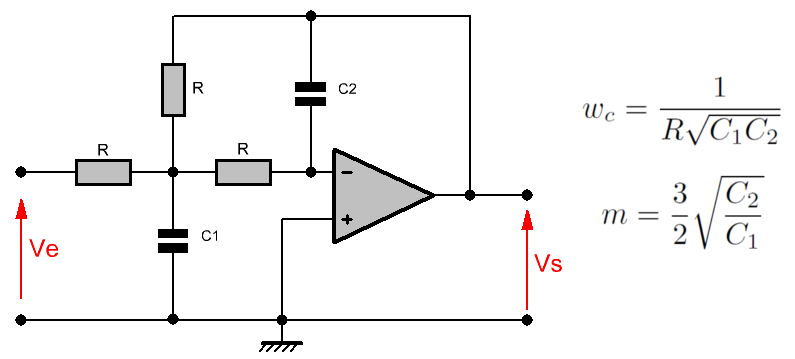
\includegraphics[scale=0.75]{images/rauch_help.png}
\end{center}

La pulsation caractéristique de ce filtre vaut $\omega_c = \frac{1}{R \cdot \sqrt{C_1 C_2}}$ et le facteur de qualité vaut $Q = \frac{1}{3} \cdot \sqrt{\frac{C_1}{C_2}}$.


\textbf{\textsc{On utilisera l'alimentation symétrique ($V_{CC} = 7V$).}}	



%%%%%%%%%%%%%%%%%%%%%%%%%%%%%%%%%%
\subsection*{B1 - Etude théorique}

Ce montage utilise un amplificateur linéaire intégré (ALI) de type \texttt{TL071}/\texttt{TL081} (voir documentation en annexe) qui fonctionne ici en régime linéaire. On a alors la relation suivante sur les entrées de l'ALI : $V+ = V-$ et les courants d'entrée $i+$ et $i-$ de cet amplificateur sont supposés nuls.

\Real Faire une étude du fonctionnement du circuit en basse et en haute fréquence. En déduire le comportement attendu de ce filtre et donner les valeurs numérique le caractérisant pour les valeurs de composants
suivantes : $R = 2.2\operatorname{k\Omega}$, $C_1 = 22\operatorname{nF}$ et $C_2 = 2.2\operatorname{nF}$.

%%%%%%%%%%%%%%%%%%%%%%%%%%%%%%%%%%
\subsection*{B2 - Etude en fréquence de cette structure}

\Real Réaliser le montage précédent avec les valeurs de composants $R = 2.2~k\Omega$, $C_1 = 22~nF$, $C_2 = 2.2~nF$. 

\Real Proposer un protocole d'étude en fréquence de ce montage.

\Real Caractériser ce système pour des fréquences allant de 10Hz à 100kHz.

\Real Analyser les résultats pour valider le comportement de ce filtre.


\subsection*{B3 - Montage complet}

\Real Justifier le rôle du filtre vis-à-vis du système de détection synchrone pour récupérer le signal modulant. Comment mettre en cascade ces deux éléments pour retrouver le signal modulant initial ?

\Real Valider le principe de la démodulation en associant les deux montages.



%%%%%%%%%%%%%%%%%%%%%%%%%%%%%%%%%%

\noindent \rule{\linewidth}{1pt}





\end{document}
